\documentclass[a4paper,14pt]{article}

\usepackage{comment} % Para comentar várias linhas ao mesmo tempo

%matemática
\usepackage{amsmath}
\usepackage{amssymb}

%diagramação
\usepackage{extsizes}
\everymath{\displaystyle}
\usepackage{geometry}
\usepackage{fancyhdr}
\usepackage{multicol}
\usepackage{graphicx}
\usepackage[brazil]{babel}
\usepackage[shortlabels]{enumitem}
\usepackage{cancel}
\usepackage{textcomp}
\usepackage{tcolorbox}

%tabelas
\usepackage{array} % Para melhor formatação de tabelas
\usepackage{longtable}
\usepackage{booktabs}  % Para linhas horizontais mais bonitas
\usepackage{float}   % Para usar o modificador [H]
\usepackage{caption} % Para usar legendas em tabelas
\usepackage{wrapfig} % Para usar tabelas e figuras flutuantes
\usepackage{xcolor} % Para cores do fundo de tabelas
\usepackage{colortbl} % Para cores do fundo de tabelas

%tikzpicture
\begin{comment}
	\usepackage{tikz}
	\usepackage{scalerel}
	\usepackage{pict2e}
	\usepackage{tkz-euclide}
	\usetikzlibrary{calc}
	\usetikzlibrary{patterns,arrows.meta}
	\usetikzlibrary{shadows}
	\usetikzlibrary{external}
\end{comment}


%pgfplots
\usepackage{pgfplots}
\pgfplotsset{compat=newest}
\usepgfplotslibrary{statistics}
\usepgfplotslibrary{fillbetween}

%colours
\usepackage{xcolor}



\columnsep=2cm
\hoffset=0cm
\textwidth=8cm
\setlength{\columnseprule}{.1pt}
\setlength{\columnsep}{2cm}
\renewcommand{\headrulewidth}{0pt}
\geometry{top=1in, bottom=1in, left=0.7in, right=0.5in}

\pagestyle{fancy}
\fancyhf{}
\fancyfoot[C]{\thepage}

\begin{document}
	
	\noindent\textbf{6FMA144 - Matemática} 
	
	\begin{center}Retas paralelas cortadas por uma transversal (Versão estudante)
	\end{center}
	
	\noindent\textbf{Nome:} \underline{\hspace{10cm}}
	\noindent\textbf{Data:} \underline{\hspace{4cm}}
	
	%\section*{Questões de Matemática}
	
	\begin{multicols}{2}
	    \noindent Considere $r$ e $s$ duas retas paralelas e $t$ uma reta transversal a elas. Temos: \\
	    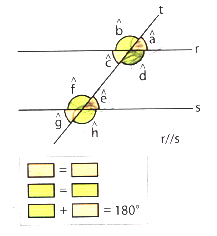
\includegraphics[width=1\linewidth]{6FMA144_imagens/imagem1} \\
	    \begin{itemize}
	    	\item \textbf{correspondentes:} $\{\hat{a}; \hat{e}\}, \{\hat{b}; \hat{f}\}, \\ \{\hat{c}; \hat{g}\}, \{\hat{d}; \hat{h}\}$;
	    	\item \textbf{alternos internos:} $\{\hat{d}; \hat{f}\}, \{\hat{c}; \hat{e}\}$;
	    	\item \textbf{alternos externos:} $\{\hat{a}; \hat{g}\}, \{\hat{b}; \hat{h}\}$;
	    	\item \textbf{colaterais internos:} $\{\hat{d}; \hat{e}\}, \{\hat{c}; \hat{f}\}$;
	    	\item \textbf{colaterais externos:} $\{\hat{a}; \hat{h}\}, \{\hat{b}; \hat{g}\}$;
	    \end{itemize}
	    
		\noindent\textsubscript{--------------------------------------------------------------------------}
		\begin{enumerate} 
			\item Determine o valor das incógnitas em cada um dos casos:
			\begin{enumerate}[a)]
				\item $r // s$ \\
				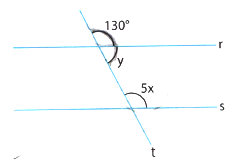
\includegraphics[width=1\linewidth]{6FMA144_imagens/imagem2} \\\\\\\\\\\\\\\\\\\\
				\item $r // s$ \\
				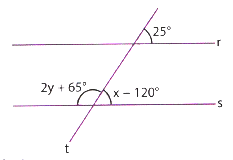
\includegraphics[width=1\linewidth]{6FMA144_imagens/imagem3} \newpage
				\item $r // s$ \\
				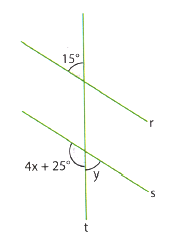
\includegraphics[width=1\linewidth]{6FMA144_imagens/imagem4} \\\\\\\\\\\\\\
				\item $r // s$ \\
				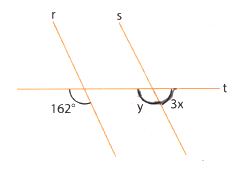
\includegraphics[width=1\linewidth]{6FMA144_imagens/imagem5} \\\\\\\\\\\\\\\\
			\end{enumerate}
			\item Sabendo que $\overline{BC}$ // $\overline{DE}$, determine os ângulos dos triângulos $ABC$ e $ADE$ em cada caso: \\
			\begin{enumerate}[a)]
				\item \begin{tabular}{|c|c|}
					\hline $\Delta$$\textbf{ABC}$
					& $\Delta$$\textbf{ADE}$ \\
					\hline
					$m(\hat{A}) = 25$° & $m(\hat{A}) = 25$° \\
					\hline
					$m(\hat{B}) = ~~~~$ & $m(\hat{D}) = ~~~~$ \\
					\hline
					$m(\hat{C}) = ~~~~$ & $m(\hat{E}) = 45$° \\
					\hline 
				\end{tabular}
				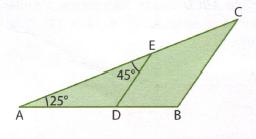
\includegraphics[width=1\linewidth]{6FMA144_imagens/imagem6} \\\\\\\\\\\\\\\\
				\item \begin{tabular}{|c|c|}
					\hline $\Delta$$\textbf{ABC}$
					& $\Delta$$\textbf{ADE}$ \\
					\hline
					$m(\hat{A}) = ~~~~$ & $m(\hat{A}) = ~~~~$ \\
					\hline
					$m(\hat{B}) = 70$° & $m(\hat{D}) = ~~~~$ \\
					\hline
					$m(\hat{C}) = ~~~~$ & $m(\hat{E}) = 30$° \\
					\hline
				\end{tabular}
				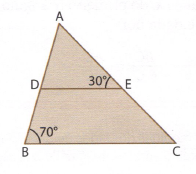
\includegraphics[width=1\linewidth]{6FMA144_imagens/imagem7} \newpage
			\end{enumerate}
			\item Na figura a seguir, determine $x$, medida do ângulo assinalado, sabendo que $\overline{DE}$ // $\overline{BC}$ e $\overline{EC}$ // $\overline{AB}$. \\
			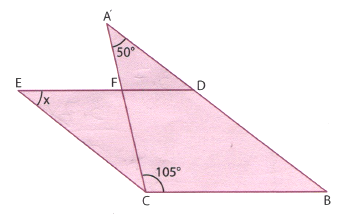
\includegraphics[width=1\linewidth]{6FMA144_imagens/imagem8} \\\\\\\\\\\\\\\\\\\\
			% 83 a 87
			\item Nos itens a seguir, sabendo que $r // s$, determine a medida de $x$, em graus:
			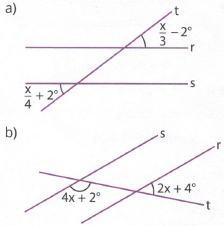
\includegraphics[width=1\linewidth]{6FMA144_imagens/imagem9} \\\\\\
			\item Na figura a seguir, sabendo que $r // s$ e $t // u$, determine as medidas de $x$ e $y$, em graus:
			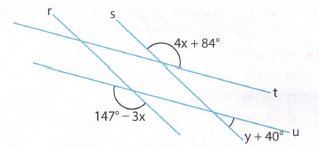
\includegraphics[width=1\linewidth]{6FMA144_imagens/imagem10} \\\\\\\\\\\\\\\\\\\\
			\item (Ufes) Uma transversal intercepta duas paralelas formando ângulos alternos internos expressos em graus por (5x + 8°) e (7x - 12°). A soma das medidas desses ângulos é:
			\begin{enumerate}[a)]
				\item 40°
				\item 58°
				\item 80°
				\item 116°
				\item 150° \newpage
			\end{enumerate}
			\item Na figura a seguir, sabendo que as retas $r$ e $s$ são paralelas, determine a medida de $x$, em graus: \\
			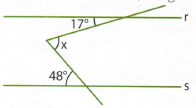
\includegraphics[width=1\linewidth]{6FMA144_imagens/imagem11} \\\\\\\\\\\\\\\\\\\\
			\item As estradas Andrômeda e Órion são paralelas, as estradas Perseu e Órion fazem um ângulo menor de 40° e as estradas Sírius e Perseu fazem um ângulo maior de 100°, de acordo com a figura a seguir. \\
			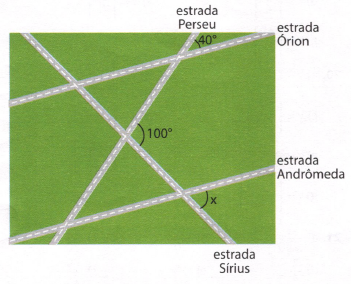
\includegraphics[width=1\linewidth]{6FMA144_imagens/imagem12}
			Qual é a medida do menor ângulo $x$ entre as estradas Andrômeda e Sírius?
		\end{enumerate}
		$~$ \\ $~$ \\ $~$ \\ $~$ \\ $~$ \\ $~$ \\ $~$ \\ $~$ \\ $~$ \\ $~$ \\ $~$ \\ $~$ \\ $~$ \\ $~$ \\ $~$ \\ $~$ \\ $~$ \\ $~$ \\ $~$ \\ $~$ \\ $~$ \\ $~$ \\ $~$ \\ $~$ \\ $~$ \\ $~$ \\ $~$ \\ $~$ \\ $~$ \\ $~$ \\ $~$ \\ $~$ \\ $~$ \\ $~$ \\ $~$ \\ $~$ \\ $~$ \\ $~$ \\ $~$ \\ $~$ \\ $~$ \\ $~$ \\ 
	\end{multicols}
\end{document}